\documentclass[11pt,a4paper]{article}
\usepackage[utf8]{inputenc}
\usepackage[T1]{fontenc}
\usepackage{lmodern}
\usepackage[ngerman]{babel}
\usepackage[a4paper,margin=2.5cm]{geometry}
\usepackage{amsmath,amssymb}
\usepackage{siunitx}
\sisetup{locale=DE, per-mode=symbol}
\usepackage{booktabs}
\usepackage{tabularx}
\usepackage[section]{placeins}
\usepackage{graphicx}
\usepackage{caption}
\captionsetup{font=small,labelfont=bf}
\usepackage[hidelinks]{hyperref}

\newcommand{\Pone}{P_{\mathrm{1dB}}}
\newcommand{\Prf}{P_{\mathrm{rf}}}
\newcommand{\Ppk}{P_{\mathrm{pk}}}
\newcommand{\Ckrit}{C_{\mathrm{krit}}}

\title{Beugungseffizienz der gekreuzten AODs\\ in Abhängigkeit vom Crestfaktor}
\author{Beating-GUI, Ein-Linsen-Aufbau}
\date{22.~September 2026}

\begin{document}
\maketitle

\begin{abstract}
\noindent
Wie viel der optischen Leistung vor dem AOD kommt im Multiton-Profil an, wenn die
Tonphasen einen bestimmten Crestfaktor $C$ erzeugen? Die Rechnung verbindet drei
Dinge: das Effizienzmodell eines AOD mit mehreren Tönen, die Grenzen der
RF-Kette für die Spitzenleistung und die Daten der eingesetzten Geräte
(AA DTSXY-400-800, Mini-Circuits ZHL-03-5WF+). Ergebnis für
$13\times14$ Töne, \SI{1,56}{\mega\hertz} Bandbreite und \SI{300}{\milli\watt}
vor dem AOD: mit Schroeder-Phasen etwa \SI{210}{\milli\watt} im Profil, mit
Phasen null nur \SI{14}{\milli\watt}. Bis $C\approx1{,}75$ kostet der Crestfaktor
kein Licht.
\end{abstract}

%======================================================================
\section{Die Geräte}

\begin{table}[htbp]
\centering\small
\begin{tabularx}{\textwidth}{@{}l>{\raggedright\arraybackslash}Xl@{}}
\toprule
Größe & Wert & Quelle\\
\midrule
AOD & AA DTSXY-400-800, TeO$_2$, \SI{36}{\mega\hertz} Bandbreite & Test Sheet\\
Mittenfrequenz, \SI{795}{\nano\meter} & \SI{103}{\mega\hertz} $\pm$\SI{4}{\mega\hertz} & Test Sheet\\
RF je Achse (Messpunkt) & \SI{1,3}{\watt} & Test Sheet\\
Effizienz eine Achse & \SIrange{83}{89}{\percent} bei \SI{1,3}{\watt} & Test Sheet, S.~3\\
Effizienz \glqq 1-1\grqq{} & \SIrange{62}{70}{\percent} (Spezifikation $>\SI{58}{\percent}$) & Test Sheet\\
max.\ mittlere RF & \SI{2}{\watt} je Achse & Test Sheet\\
Sättigung $\beta$ & \SIrange{1,4}{1,8}{\watt} (anderes Exemplar, \SI{799,5}{\nano\meter}) & \cite[Abb.~3.8]{mittenbuehler}\\
Spitzen-RF-Grenze & \SI{4}{\watt} (Laborpraxis) & \cite[Abschn.~3.3]{mittenbuehler}\\
\midrule
Verstärker & Mini-Circuits ZHL-03-5WF+, \SIrange{60}{300}{\mega\hertz}, \SI{30}{\deci\bel} & \cite{zhl}\\
$\Pone$ & \SI{+36}{dBm} typ.\ $=\SI{3,98}{\watt}$ & \cite{zhl}\\
OIP3 & \SI{+49}{dBm} & \cite{zhl}\\
\bottomrule
\end{tabularx}
\caption{Eingangsdaten. Test Sheet: AA Opto-Electronic, S/N 3001-O211386 \cite{testsheet}. Mittenbühler nennt für den Verstärker \SI{+39}{dBm}
($\SI{8}{\watt}$) bei \SI{1}{\deci\bel} Kompression; das Datenblatt sagt
\SI{+36}{dBm}. Hier wird das Datenblatt verwendet.}
\label{tab:geraete}
\end{table}

%======================================================================
\section{Beugung eines Tons: was $\alpha$ und $\beta$ sind}

Die RF-Leistung $P$ erzeugt im Kristall eine Schallwelle. Deren Dehnung
moduliert den Brechungsindex; die Amplitude dieser Modulation wächst wie
$\sqrt{P}$, denn Leistung ist quadratisch in der Amplitude. Im Bragg-Regime
tauschen einfallende und gebeugte Welle entlang des Kristalls periodisch
Leistung aus, und am Ausgang ist der gebeugte Anteil ein Sinusquadrat dieser
Kopplung. Mit der Näherung ohne Impulsfehlanpassung, deren Rest in einen
Vorfaktor gesteckt wird, lautet das Ergebnis
\cite[Gl.~3.12]{mittenbuehler}
\begin{equation}
  \eta(P) \;=\; \alpha\,\sin^2\!\left(\frac{\pi}{2}\sqrt{\frac{P}{\beta}}\right).
  \label{eq:eta1}
\end{equation}
Die beiden Parameter haben eine unmittelbar ablesbare Bedeutung
(Abb.~\ref{fig:etaP}):

\begin{description}
\item[$\alpha$ -- Spitzeneffizienz.] Der größte Anteil des einfallenden Lichts,
  den \emph{eine} AOD-Achse überhaupt in die erste Ordnung beugen kann. Er
  liegt unter eins, weil die Bragg-Bedingung nicht über die ganze Bandbreite
  exakt erfüllt ist, das Strahlprofil nicht ideal ist und Reflexe verloren
  gehen. $\alpha$ ist die \emph{Höhe} des Maximums. Aus dem Test Sheet: eine
  Achse erreicht bei \SI{1,3}{\watt} \SIrange{83}{89}{\percent}, also
  $\alpha\approx0{,}85$.
\item[$\beta$ -- Sättigungsleistung.] Die RF-Leistung, bei der dieses Maximum
  erreicht wird: bei $P=\beta$ ist das Argument des Sinus genau $\pi/2$. $\beta$
  ist die \emph{Lage} des Maximums. Mehr Leistung bringt kein Licht mehr, sie
  koppelt es zurück in den ungebeugten Strahl. Der Arbeitspunkt des Test
  Sheets, \SI{1,3}{\watt}, liegt im Maximum; Mittenbühler findet für ein
  anderes Exemplar desselben Typs \SIrange{1,4}{1,8}{\watt}, abhängig von
  Frequenz und Achse. Hier: $\beta=\SI{1,3}{\watt}$.
\end{description}

Zwei Grenzfälle machen die Rollen deutlich. Für kleine Leistung ist
$\eta\approx\alpha(\pi/2)^2\,P/\beta$ -- linear in $P$, mit Steigung
$\alpha/\beta$. Bei $P=\beta$ ist $\eta=\alpha$. Die Schreibweise
$\sin^2(\kappa\sqrt{P})$ aus \cite[Gl.~181]{crest} ist dieselbe Kurve mit
$\kappa=\pi/(2\sqrt{\beta})$ und $\alpha=1$.

\begin{figure}[htbp]
  \centering
  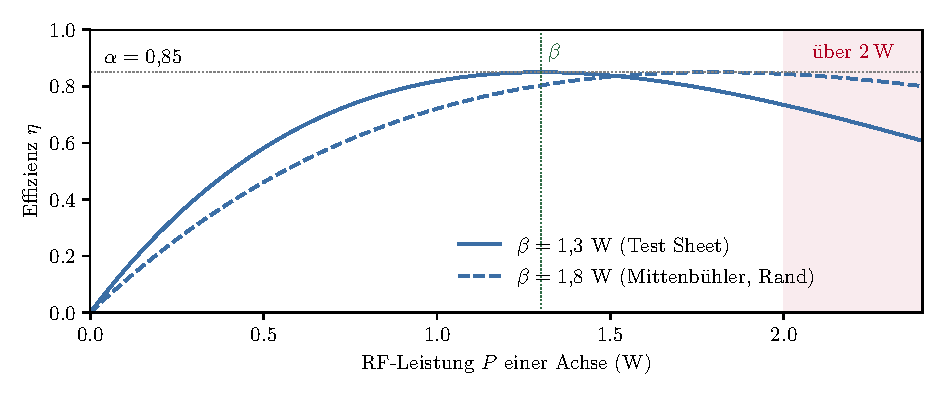
\includegraphics[width=\textwidth]{beugung_eta_P.pdf}
  \caption{Gl.~\eqref{eq:eta1} für eine Achse. $\alpha$ ist die Höhe,
  $\beta$ die Lage des Maximums. Gestrichelt: $\beta=\SI{1,8}{\watt}$ am oberen
  Rand der Werte aus \cite{mittenbuehler}. Oberhalb von \SI{2}{\watt} ist der
  Wandler thermisch überlastet.}
  \label{fig:etaP}
\end{figure}

%======================================================================
\section{Mehrere Töne: nur die Gesamtleistung zählt}

Mit $N$ Tönen der Leistungen $P_n$ stehen $N$ Gitter gleichzeitig im Kristall,
und alle speisen sich aus \emph{derselben} ungebeugten Welle. Die gekoppelten
Gleichungen reduzieren sich exakt auf ein Zwei-Wellen-System mit der
Kopplung $\sqrt{\sum_n P_n}$ \cite[Gl.~3.20--3.25]{mittenbuehler},
\cite[Gl.~190--200]{crest}. Damit
\begin{equation}
  \eta_\mathrm{ges} = \alpha\,\sin^2\!\left(\frac{\pi}{2}\sqrt{\frac{\Prf}{\beta}}\right),
  \qquad
  \eta_n = \eta_\mathrm{ges}\,\frac{P_n}{\Prf},
  \qquad
  \Prf=\sum_n P_n .
  \label{eq:etaN}
\end{equation}
Die Summe steht unter der Wurzel, nicht vor den Sinusquadraten: Ein weiterer Ton
öffnet keinen neuen Kanal, er teilt den vorhandenen. Die Aufteilung eines
Profils auf viele Töne kostet daher bei gleicher Gesamtleistung keine Effizienz.

\paragraph{Die Tonphasen kommen nicht vor.} Jeder Ton ist eine Fourierkomponente
des Schallfelds mit konstanter Amplitude; seine Phase verschiebt nur die Lage
seines Gitters und taucht als Phase der gebeugten Welle wieder auf -- im
Interferenzbild, nicht in $\eta_n$. Der Crestfaktor wirkt deshalb nicht über die
Beugung, sondern allein darüber, \emph{wie viel} RF-Leistung die Kette linear
liefern darf.

%======================================================================
\section{Wie viel RF-Leistung darf in eine Achse?}

Der Crestfaktor des reellen RF-Signals $s(t)$ einer Achse ist
$C=\max_t|s|/s_\mathrm{rms}$. An der Last $R$ ist die mittlere Leistung
$\Prf=s_\mathrm{rms}^2/R$ und die momentane Spitzenleistung
\begin{equation}
  \Ppk = \frac{\max_t s^2}{R} = C^2\,\Prf .
  \label{eq:ppk}
\end{equation}
Für einen einzelnen Ton ist $C=\sqrt2$ und $\Ppk=2\Prf$; mit Phasen null und
$N$ gleichen Tönen ist $C=\sqrt{2N}$.

Vier Grenzen begrenzen $\Prf$; die kleinste gewinnt.

\begin{enumerate}
\item \textbf{Verstärker, Linearität.} $\Pone$ ist die \emph{mittlere} Leistung
  eines Dauerstrich-Tons, bei der die Verstärkung um \SI{1}{\deci\bel} eingebrochen
  ist. Die Momentanspitze dieses Tons ist $2\Pone$. Maßgeblich für ein
  Mehrtonsignal ist die Spitzenhüllkurvenleistung
  $\mathrm{PEP}=\Ppk/2$; die Bedingung $\mathrm{PEP}\le\Pone$ ergibt
  \begin{equation}
    \Ppk \le 2\Pone = \SI{7,96}{\watt}
    \quad\Longrightarrow\quad
    \Prf \le \frac{2\Pone}{C^2}.
    \label{eq:amp}
  \end{equation}
\item \textbf{AOD, Spitze.} Das Handbuch erlaubt \SI{2}{\watt} mittlere
  Einzelton-Leistung. Mittenbühler leitet daraus als Schutzgrenze eine
  Momentanspitze von \SI{4}{\watt} ab \cite[Abschn.~3.3]{mittenbuehler}:
  \begin{equation}
    \Ppk \le \SI{4}{\watt}
    \quad\Longrightarrow\quad
    \Prf \le \frac{\SI{4}{\watt}}{C^2}.
    \label{eq:aodpk}
  \end{equation}
  Das ist Laborpraxis, kein Datenblattwert.
\item \textbf{AOD, thermisch.} $\Prf\le\SI{2}{\watt}$.
\item \textbf{Sättigung.} $\Prf\le\beta$; mehr bringt kein Licht.
\end{enumerate}
Zusammen:
\begin{equation}
  \Prf = \min\!\left(\beta,\; \SI{2}{\watt},\; \frac{\min(2\Pone,\;\SI{4}{\watt})}{C^2}\right).
  \label{eq:prf}
\end{equation}
Mit den Daten aus Tab.~\ref{tab:geraete} greift die AOD-Spitze (\SI{4}{\watt})
vor dem Verstärker (\SI{7,96}{\watt}). Solange
\begin{equation}
  C \le \Ckrit = \sqrt{\frac{\SI{4}{\watt}}{\beta}} = 1{,}75,
  \label{eq:ckrit}
\end{equation}
ist die Sättigung die Grenze, und der Crestfaktor kostet kein Licht. Darüber
fällt $\Prf$ wie $1/C^2$ und mit ihm die Effizienz nach Gl.~\eqref{eq:etaN}
(Abb.~\ref{fig:etaC}).

%======================================================================
\section{Zwei Achsen und die Leistung im Profil}

Jeder Spot $(n,m)$ wird einmal im $x$- und einmal im $y$-AOD gebeugt. Über alle
Spots summiert faktorisiert die Effizienz der Ordnung \glqq 1-1\grqq:
\begin{equation}
  \sum_{n,m}\eta_{x,n}\,\eta_{y,m} = \eta_x\,\eta_y,
  \qquad
  P_\mathrm{Profil} = P_\mathrm{in}\,\eta_x\,\eta_y .
  \label{eq:profil}
\end{equation}
Mit $\alpha=0{,}85$ je Achse ergibt das bei voller Aussteuerung $0{,}72$; das Test
Sheet misst für beide Achsen zusammen \SIrange{62}{70}{\percent}. Die Differenz
passt zu dem Kopplungsterm $\Xi$ gekreuzter AODs, der die Effizienz zum Rand des
Frequenzbereichs hin senkt \cite[Gl.~3.28]{mittenbuehler}; in der Bandmitte, wo
das $13\times14$-Profil liegt, ist er nahe eins.

\begin{figure}[htbp]
  \centering
  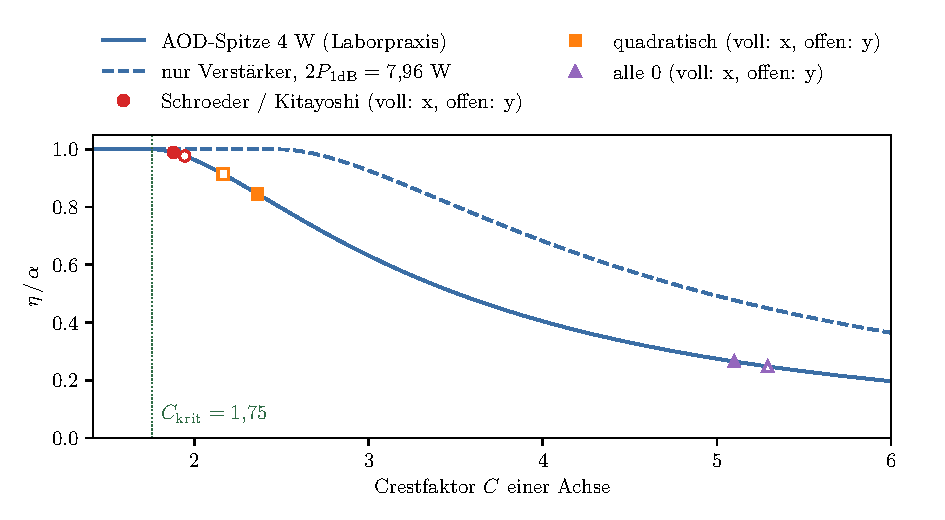
\includegraphics[width=\textwidth]{beugung_eta_C.pdf}
  \caption{Effizienz einer Achse relativ zu $\alpha$ über dem Crestfaktor,
  $\beta=\SI{1,3}{\watt}$. Durchgezogen mit der AOD-Spitzengrenze
  \SI{4}{\watt}, gestrichelt nur mit der Verstärkergrenze $2\Pone$. Marker:
  Crestfaktoren der Phasensätze für $13\times14$ Töne.}
  \label{fig:etaC}
\end{figure}

%======================================================================
\section{Zahlen für den Ein-Linsen-Aufbau}

$13\times14$ Töne, gleiche Amplituden, width \SI{1,56}{\mega\hertz},
$P_\mathrm{in}=\SI{300}{\milli\watt}$, $\alpha=0{,}85$, $\beta=\SI{1,3}{\watt}$,
Spitzengrenze \SI{4}{\watt}:

\begin{table}[htbp]
\centering\small
\begin{tabular}{lcccccc}
\toprule
Phasen & $C_x$ & $C_y$ & $P_{\mathrm{rf},x/y}$ (W) & $\eta_x$ / $\eta_y$ (\%) & $\eta_x\eta_y$ & $P_\mathrm{Profil}$\\
\midrule
alle 0            & 5,10 & 5,29 & 0,15 / 0,14 & 22 / 21 & \SI{4,7}{\percent} & \SI{14}{\milli\watt}\\
Schroeder         & 1,88 & 1,94 & 1,13 / 1,06 & 84 / 83 & \SI{69,8}{\percent} & \SI{209}{\milli\watt}\\
Kitayoshi         & 1,88 & 1,94 & 1,13 / 1,06 & 84 / 83 & \SI{69,8}{\percent} & \SI{209}{\milli\watt}\\
$2\pi n(n-1)/(N-1)$ & 2,36 & 2,16 & 0,72 / 0,85 & 72 / 78 & \SI{55,8}{\percent} & \SI{167}{\milli\watt}\\
symm.\ optimiert ($C\le1{,}9$) & 1,89 & 1,89 & 1,12 / 1,12 & 84 / 84 & \SI{70,4}{\percent} & \SI{211}{\milli\watt}\\
\bottomrule
\end{tabular}
\caption{Effizienz und Leistung im Profil (vor der Optik hinter den AODs). In
allen Zeilen begrenzt die AOD-Spitze.}
\label{tab:zahlen}
\end{table}

\paragraph{Wie empfindlich sind die Zahlen?} $\beta$ ist für dieses Exemplar nicht
gemessen, und die \SI{4}{\watt} sind eine Schutzgrenze. Tab.~\ref{tab:sens}
variiert beides.

\begin{table}[htbp]
\centering\small
\begin{tabular}{lccccc}
\toprule
& & & \multicolumn{3}{c}{$P_\mathrm{Profil}$ (mW)}\\
\cmidrule(lr){4-6}
$\beta$ & Spitzengrenze & $\Ckrit$ & Schroeder & quadratisch & alle 0\\
\midrule
\SI{1,3}{\watt} & \SI{4}{\watt}   & 1,75 & 209 & 167 & 14\\
\SI{1,5}{\watt} & \SI{4}{\watt}   & 1,63 & 195 & 146 & 11\\
\SI{1,8}{\watt} & \SI{4}{\watt}   & 1,49 & 170 & 118 & 8\\
\SI{1,3}{\watt} & $2\Pone$ = \SI{7,96}{\watt} & 2,47 & 217 & 217 & 46\\
\SI{1,8}{\watt} & $2\Pone$ = \SI{7,96}{\watt} & 2,10 & 217 & 210 & 27\\
\bottomrule
\end{tabular}
\caption{Leistung im Profil für andere $\beta$ und ohne die AOD-Spitzengrenze
($P_\mathrm{in}=\SI{300}{\milli\watt}$).}
\label{tab:sens}
\end{table}

%======================================================================
\section{Was nicht enthalten ist}

\begin{itemize}
\item \textbf{Intermodulation.} Nach der Zwei-Ton-Regel liegen die Produkte
  dritter Ordnung des Verstärkers bei \SI{19,4}{dBm} je Ton
  ($\SI{1,13}{\watt}/13$) etwa $2(\mathrm{OIP3}-P_\mathrm{Ton})\approx
  \SI{59}{dBc}$ unter den Tönen. Mit vielen Tönen addieren sich viele Produkte;
  Mittenbühler misst bei 40 Tönen \SI{-27}{\deci\bel} im Verstärker und
  \SI{-18}{\deci\bel} im AOD selbst (bei etwa \SI{50}{\percent} Effizienz), bei
  10 Tönen im AOD keine sichtbaren Nebenspots \cite[Abschn.~2.3, 3.3.4]{mittenbuehler}.
  Bei 13 und 14 Tönen ist ein Verlust im Prozentbereich zu erwarten; die Zahlen
  in Tab.~\ref{tab:zahlen} sind daher eher Obergrenzen.
\item \textbf{Phasenanpassung über die Tonspanne.} Der äußerste Ton liegt
  \SI{0,78}{\mega\hertz} neben der Mitte. Mit der Eichung \glqq Effizienz auf die
  Hälfte am Bandrand, \SI{18}{\mega\hertz}\grqq{} aus \cite[Gl.~202--203]{crest}
  kostet das \SI{0,1}{\percent}.
\item \textbf{Kopplung der gekreuzten AODs} $\Xi$ (siehe oben), Frequenzgang von
  $\alpha$ und $\beta$, Kabel- und Filterverluste, Transmission der Optik hinter
  den AODs.
\end{itemize}

%======================================================================
\section{Abgleich mit der Crestfaktor-Ausarbeitung}

\begin{enumerate}
\item Gl.~(174) dort verlangt $C^2\Prf\le\Pone$, vergleicht also die
  Momentanspitze mit einer Dauerstrich-\emph{Mittel}\-leistung. Nach
  Gl.~\eqref{eq:amp} ist die zulässige Leistung doppelt so groß,
  $\Prf\le2\Pone/C^2$. Am Aufbau ändert das wenig, weil die AOD-Spitze zuerst
  greift.
\item Abschnitt~9.5 dort setzt $\alpha=1$ und eicht $\kappa$ an den \glqq$>\SI{58}{\percent}$\grqq{}
  beider Achsen, also \SI{76}{\percent} je Achse bei \SI{1,3}{\watt}; die
  Sättigung läge dann erst bei \SI{2,85}{\watt}. Die Einzelachsen-Kurve des Test
  Sheets (\SIrange{83}{89}{\percent} bei \SI{1,3}{\watt}) und die $\beta$-Werte
  von Mittenbühler sprechen für $\alpha<1$ und $\beta$ zwischen \SI{1,3}{\watt}
  und \SI{1,8}{\watt}. Bei \SI{0,664}{\watt} gibt Gl.~\eqref{eq:eta1}
  $\eta=0{,}69$ statt $0{,}47$.
\item Abschnitt~9.1 dort behandelt die \SI{2}{\watt} nur als thermische Grenze.
  Die zusätzliche Spitzengrenze von \SI{4}{\watt} aus der Laborpraxis ist hier
  die bindende.
\end{enumerate}

{\sloppy\paragraph{Umsetzung.} Gl.~\eqref{eq:etaN} und \eqref{eq:prf} stehen als Funktion
\texttt{aod\_drive()} in Abschnitt~15 von \texttt{kern/\allowbreak beating\_physik.py}. Das
Beating-GUI zeigt das Ergebnis live neben dem Crestfaktor und speichert es beim
Export als eigene Seite \texttt{\_diffraction.pdf} und im Parameter-Text.\par}

\begin{thebibliography}{9}
\bibitem{mittenbuehler} M.~Mittenbühler, \emph{Reactive Real-Time Synthesis of
  Multiple Tweezers for Parallelized Atom Transport}, Masterarbeit, TU Darmstadt
  (2024).
\bibitem{crest} \emph{Der Crestfaktor als Randbedingung bei der Wahl der Tonphasen}, interne
  Ausarbeitung, Stand 22 (September 2026).
\bibitem{testsheet} AA Opto-Electronic, Test Sheet DTSXY-400-800, S/N
  3001-O211386 (12.04.2022).
\bibitem{zhl} Mini-Circuits, Datenblatt ZHL-03-5WF+,
  \url{https://www.minicircuits.com/pdfs/ZHL-03-5WF+.pdf}.
\end{thebibliography}

\end{document}
